% !TEX encoding = UTF-8 Unicode

\documentclass[a4paper]{article}

\usepackage{color}
\usepackage{url}
\usepackage{amsthm}
\usepackage[T2A]{fontenc} % enable Cyrillic fonts
\usepackage[utf8]{inputenc} % make weird characters work
\usepackage{graphicx}
\graphicspath{ {img/} }

\usepackage[english,serbian]{babel}
%\usepackage[english,serbianc]{babel} %ukljuciti babel sa ovim opcijama, umesto gornjim, ukoliko se koristi cirilica

\usepackage[unicode]{hyperref}
\hypersetup{colorlinks,citecolor=green,filecolor=green,linkcolor=blue,urlcolor=blue}

\newtheorem*{tvrdjenje}{Tvrđenje}
\theoremstyle{definition}
%\newtheorem{primer}{Пример}[section] %ćirilični primer
\newtheorem{primer}{Primer}[section]


\begin{document}

%\renewcommand{\abstractname}{Apstrakt} %pisace Sazetak ako se ne ukljuci ova naredba

\title{Primena mašinskog učenja u verifikaciji softvera\\ \small{Seminarski rad u okviru kursa\\Metodologija stručnog i naučnog rada\\ Matematički fakultet}}

\author{Nikola Dimitrijević, Rastko Đorđević,\\
 Luka Živanović, Dimitrije Špadijer\\
 nikoladim95@gmail.com, mi14078@alas.matf.bg.ac.rs,\\
  mi14164@alas.matf.bg.ac.rs, mm11021@alas.matf.bg.ac.rs}
%\date{9.~april 2015.}
\vspace*{-3cm}
    {\let\newpage\relax\maketitle}

\abstract{
Verifikacija softvera je izuzetno važna oblast računarstva. Softver polako uspeva da se uplete u najneočekivanije aspekte naših života i zbog toga njegova ispravnost postaje od sve većeg značaja. Neispravan softver može imati katastrofalne posledice, koje uključuju i izgubljene ljudske živote. Sa druge strane, tehnike mašinskog učenja se ubrzano u\-sa\-vr\-ša\-va\-ju i neprekidno uspevaju da ostvare iznenađujuće dobre rezultate u svim oblastima računarstva. U ovom radu biće predstavljeni neki od bitnijih pomaka u sudaru pomenutih oblasti sa ciljem da zainteresuje što veći broj ljudi da se pridruže pohodu za sprečavanje bagova korišćenjem modernih tehnika mašinskog učenja.

%Molim Vas da kada budete predavali seminarski rad, imenujete datoteke tako da sadrže temu seminarskog rada, kao i imena i prezimena članova grupe (ili samo temu i prezimena, ukoliko je sa imenima predugačko). Predaja seminarskih radova biće isključivo preko web forme, a NE slanjem mejla.}

\tableofcontents

\newpage



% ==============================================================================
\section{Uvod}
\label{sec:uvod}
% ==============================================================================

\par Računarska rešenja se koriste za svemirske rakete, medicinsku opremu, samovozeće automobile i u raznim drugim oblastima. Sve veća zastupljenost i složenost softvera dovodi do veće verovatnoće katastrofalnog ishoda u slučaju greške. Privremena nedostupnost vlastitog novca, pad satelita, prekomerno doziranje terapije pacijentima i puštanje nasilnih zatvorenika na slobodu su primeri stvarnih događaja usled grešaka u programima.

\par Verifikacija softvera je oblast računarstva koja se bavi analizom soft\-ve\-ra i ispitivanjem ispravnosti programskog koda. Postoje razni alati za verifikaciju koji se uspešno koriste, ali postoje i mnoga ograničenja u procesu analize koda koje je teško prevazići, a neke je čak i nemoguće prevazići. Analiziranje programskog koda se zasniva na formalnim matematičkim modelima koje je teško automatizovati. Mašinsko učenje je postalo vrlo popularno i to sa pravom, jer ima velike uspehe u raznim domenima, pa je i prirodno nalaziti njegove primene u okviru verifikacije softvera. Ovaj rad se nastavlja na \cite{micovic} pa ovde neće biti prikazane već pomenute primene algoritama mašinskog učenja.

\par U nastavku je dat opis verifikacije soft\-ve\-ra, mašinskog učenja, i konačno pregled konkretnih primena mašinskog učenja, kako u statičkoj, tako i u dinamičkoj verifikaciji softvera.

% ==============================================================================
\section{Verifikacija softvera}
\label{sec:verifikacija}
% ==============================================================================

\par U savremenom dobu, računari i računarski sistemi predstavlju sastavni deo svakodnevice, kako u privatnom životu, tako i u poslovnom svetu, a i u državnoj administraciji. Zato je od izuzetnog značaja da softver koji se koristi bude pouzdan. Neispravan softver, u zavisnosti od toga gde se koristio i koliko je veliki bio propust, može izazvati male probleme, ali i ogromne probleme sa teškim posledicama (čak i smrtnim). Oblast razvoja softvera koja se bavi proverom ispravnosti softvera, odnosno potvrđivanjem da softver radi u skladu sa zahtevima, naziva se \emph{verifikacija softvera}.

\par Potrebno je precizirati šta se podrazumeva pod ispravnim softverom. Razlikuju se pojmovi potpuno ispravnog i delimično ispravnog softvera. Softver se smatra potpuno ispravnim ako se zaustavlja za svaki ulaz i na izlazu daje ispravan rezultat, dok se delimično ispravnim softverom smatra onaj koji za ulaz daje ispravan rezultat ako se zaustavlja, a dozvoljeno je da se za neki ulaz program ne zaustavlja. Ne postoji algoritamski način da se proveri da li se neki program zaustavlja (eng.~{\em halting problem}), pa se često ni ne ispituje potpuna, već samo delimična ispravnost softvera.

\par Postoje dve osnovne vrste verifikacije softvera i to su dinamička i statička verifikacija softvera \cite{milena}.

\subsection{Dinamička verifikacija softvera}
\label{subsec:dinamicka}

\par Dinamička verifikacija softvera zasnovana je na tome da se provera ispravnosti softvera vrši tokom njegovog izvršavanja. Najčešće se dinamička verifikacija softvera vrši testiranjem i ti pojmovi se poistovećuju, što nije sasvim ispravno.

\par Testiranje je složen proces koji obuhvata pronalaženje što raznovrsnijeg skupa ulaza, definisanje očekivanih izlaza za svaki od tih ulaza, a zatim izvršavanje programa i provera da li je program za date ulaze vratio odgovarajuće izlaze. Postoje razne vrste i nivoi testova (da li imamo pristup izvornom kodu softvera ili ne, kao i da li testiramo jednu jedinicu koda ili više njih ili testiramo neku funkcionalnost softvera).

\par Testiranje služi da, u slučaju kada postoji greška u izvornom kodu softvera, ukaže na njeno postojanje. U zavisnosti od vrste testa, kao i nivoa, može se otkriti gde se u kodu nalazi greška, ali to često nije slučaj. Umesto toga, testovi samo otkrivaju postojanje grešaka.

\par Važno je imati na umu da testovi mogu dokazati isključivo neispravnost softvera, ali ne i njegovu ispravnost. Da bi testiranje moglo dokazati delimičnu ili potpunu ispravnost softvera, neophodno bi bilo da skup ulaza bude jednak skupu svih teoretski dozvoljenih ulaza, a to, naravno, nije moguće, jer je taj skup beskonačan. Postavlja se pitanje zašto se onda uopšte testira. Odgovor je zato što se pažljivim odabirom skupa ulaza za koji će biti testirana ispravnost izlaza ne samo otklanjaju postojeće greške, nego i stiče sigurnost, odnosno poverenje u sam softver, tj. očekuje se da će broj neotkrivenih grešaka biti zanemarljiv.

\par Kao što je rečeno, često se dinamička verifikacija softvera poistovećuje sa testiranjem, iako je testiranje samo jedan od metoda. Pored testiranja postoji i debagovanje i ono očigledno spada u vid dinamičke verifikacije softvera. Naime, debagovanjem se može prekinuti rad programa u bilo kom trenutku i utvrditi trenutno stanje programa, a samim tim i potencijalno postojanje greške. Za razliku od testiranja koje se može vršiti i bez posedovanja izvornog koda softvera, debagovanje se vrši isključivo uz posedovanje koda, a često se može pronaći i tačno mesto na kome se nalazi greška.

\subsection{Statička verifikacija softvera}
\label{subsec:staticka}

\par Za razliku od dinamičke verifikacije softvera, \textit{statička verifikacija} podrazumeva analizu ispravnosti softvera bez njegovog pokretanja. Osnovna podela statičke verifikacije je na \textit{pregled koda} (eng.~{\em code review}) i na \textit{automatizovanu verifikaciju}, koja će biti ključna za ostatak rada i biće podrazumevana kada se navodi pojam statička verifikacija.

\par Kao što je već pomenuto, ne postoji način da se za svaki program utvrdi da li se on zaustavlja ili ne, tako da nam i statička verifikacija ne može uvek dati željeni odgovor. Ipak, statička verifikacija može da nam da uvid u kvalitet koda i njegove propuste za mnoge netrivijalne probleme i zbog toga se razvijaju tehnike kojim bi skup takvih problema rastao, a vreme obrade se smanjivalo. 

\par Neke od bitnijih tehnika statičke verifikacije su:
\begin{itemize}
\item \textbf{Analiza toka podataka} (eng.~{\em data flow analysis})
\item \textbf{Apstraktna interpretacija} (eng.~{\em abstract interpretation})
\item \textbf{Simbolička analiza} (eng.~{\em symbolic analysis})
\item \textbf{Proveravanje ograničenih modela} (eng.~{\em Bounded model che\-cking}), koja se najviše koristi za verifikaciju logičkih kola.
\end{itemize}

% TODO opisati tehnike koje smo koristili dole

% ==============================================================================
\section{Mašinsko učenje}
% ==============================================================================

\par \textit{Mašinsko učenje} bavi se proučavanjem indukcije, odnosno generalizacije, čime formalizuje uopštavanje od uzorka određene veličine ka univerzalnim zaključcima \cite{bishopML}. U srcu novog zamaha veštačke inteligencije nalazi se oblast mašinskog učenja. U nekim domenima, kao na primer prepoznavanje lica, u kojima se računari nisu mogli porediti sa ljudima po uspešnosti, ova oblast postiže rezultate superiorne u odnosu na rezultate ljudskih eksperata.

% TODO mozda ubaciti ovo, izbaciti nesto drugo
% Mašinsko učenje predstavlja automatsku detekciju smislenih šablona u podacima.

\par Mašinsko učenje je posebno pogodno za probleme koje je čoveku teško definisati a izuzetno lako za rešiti i u kojima je prihvatljiva poneka greška. Zbog dopuštanja povremenih grešaka u izvršavanju, ova oblast na prvi pogled izgleda kao nepogodna za rešavanje problema statičke verifikacije softvera. Ipak u stanju je da doprinese kao dodatni alat za rešavanje raznih problema koji se mogu naći u statičkoj verifikaciji ako njime rukuje prava osoba, čak i ako ne može da obeća kompletno rešenje svih problema.

\par Obično se identifikuju tri oblasti mašinskog učenja: \textit{nadgledano učenje} (eng. \emph{supervised learning}), \textit{nenadgledano učenje} (eng. \emph{unsupervised learning}) i \textit{učenje uslovljavanjem} (eng. \emph{reinforcement learning}). Nadgledano učenje odlikuje da pored ulaznih podataka postoji i njemu odgovarajući željeni izlaz. Model je zadužen za učenje pravila nad datim parovima ulaza i izlaza. Sa druge strane, kod nenadgledanog učenja dati su samo ulazni podaci pri čemu na algoritmu ostaje da pronađe strukturu u podacima. 
% TODO da li je naredna recenica suvisna (ne sme pasus da ima samo jednu recenicu, zato spojih sa gornjim)
Učenje uslovljavanjem se može videti kao oblast između dve pret\-hod\-no pomenute oblasti. U okviru učenja uslovljavanjem mora se rešiti problem preduzimanjem niza akcija, koje su međusobno povezane, kako bi se maksimizovala konačna nagrada.

\par Uobičajeni tok uspešne primene tehnika mašinskog učenja je sledeći. Nakon što se problem analizira, kao i podaci nad kojim će tehnike biti primenjene, potrebno je izabrati odgovarajući model. Nakon odabira modela, podaci se pretprocesiraju i izabrani model se trenira nad tako obrađenim podacima. Istrenirani model je dalje neophodno evaluirati kako bi bilo moguće znati u kojoj meri je koristan.

%\subsection{Odabrani algoritmi}



\subsection{Evaluacija modela i mere kvaliteta}

%TODO da li je naredna rečenica suvišna? (ne sme pasus samo 1 recenicu)
%Ukratko će biti predstavljeni termini vezani za \textit{meru kvaliteta} modela, 
%kako bi bilo olakšano razumevanje postignutih rezultata u ostatku rada.

\par \textit{Evaluacija modela} predstavlja numeričko predstavljanje sposobnosti predviđanja datog modela na određenoj skali i direktno se oslanja na mere kvaliteta. Mere koje se najčešće sreću u klasifikaciji su \textit{tačnost}, \textit{preciznost}, \textit{odziv} i \textit{F1 mera}. Sve navedene mere izvedene su iz \textit{matrice konfuzije} \ref{table:matrica_konfuzije}.

\begin{table}[h]
	\centering
	\begin{tabular}{ |c|cc| } 
		\hline
		Stvarno / Predviđeno & Pozitivno & Negativno \\ 
		\hline
		Pozitivno & Stvarno Pozitivno & Lažno Negativno \\ 
		Negativno & Lažno Pozitivno & Stvarno Negativno \\ 
		\hline
	\end{tabular}
	\caption{Matrica konfuzije}
	\label{table:matrica_konfuzije}
	%\caption{ tabelica stagod}
\end{table}

\par Stvarno pozitivne i stvarno negativne instance su one instance koje su ispravno određene od strane modela. Lažno pozitivne instance su negativne instance za koje je od strane modela predviđeno da su pozitivne, dok su lažno negativne instance zapravo pozitivne instance koje je model loše klasifikovao kao negativne. 

% TODO dodati šta koje mere zapravo rade, zašto tačnost nije savršena, napomenuti da ima još raznih
\par Tačnost klasifikacije predstavlja procenat uspešno klasifikovanih instanci u odnosu na ukupan broj instanci. Preciznost je udeo ispravno pronađenih pozitivnih instanci u svim instancama koje su proglašene za pozitivne. Odziv je udeo ispravno pronađenih pozitivnih instanci u svim zaista pozitivnim instancama. Preciznost i odziv su dve mere koje najviše ima smisla razmatrati zajedno i način na koji se to najčešće radi je F1 mera, koja predstavlja njihovu harmonijsku sredinu.

% ==============================================================================
\section{Odabrani problemi statičke verifikacije}
\label{sec:naslovN}
% ==============================================================================

\par Iako na prvi pogled mašinsko učenje možda nije očigledan odgovor na probleme koje postavlja statička verifikacija, tokom prethodnih decenija su sa razvojom mašinskog učenja postignuti izuzetno značajni uspesi u spajanju ovih oblasti. U nastavku sledi opis nekih od tih uspeha. Od uvoda u formalnu verifikaciju koji služi kao osnova mnogih daljih istraživanja, preko učenja statičkog analizatora u okviru kojeg se koriste najmodernije tehnike kako mašinskog učenja tako i testiranja, do pravljenja inteligentnog metoda detekcije grešaka koji obuhvata širok dijapazon tehnika mašinskog učenja.

\subsection{Formalna verifikacija softvera}
\label{subsec:formalna-verifikacija}

\par Verifikaciji softvera može se pristupiti na strogo formalan matematički način. U ovom radu biće izložen pristup o kome se detaljnije može pročitati u radu \cite{verify}.

\par Ako je $T$ skup testova, onda je program $P$ ispravan u odnosu na datu specifikaciju $S$ ako i samo ako važi
$$(\forall t\in T)\ [prolazi(P,t)\wedge S\models t]\Rightarrow P\equiv S,$$
gde $prolazi(P,t)$ označava da program $P$ uspešno prolazi test $t$, $S\models t$ označava da je $t$ semantička posledica specifikacije $S$, odnosno da je test u skladu sa specifikacijom programa, a $P\equiv S$ označava da se program $P$ smatra ekvivalentnim specifikaciji $S$. Drugim rečima, program je ispravan u skladu sa specifikacijom $S$ ako i samo ako se iz činjenice da program zadovoljava svaki test koji je u skladu sa specifikacijom može zaključiti da se program smatra ekvivalentnim specifikaciji.

\par Jedan od problema jeste pronaći skup testova $T$ za koji važi prethodna implikacija. Takav skup testova naziva se \emph{adekvatnim} skupom testova. Naravno, trivijalan primer je iscrpan skup testova, tj. skup testova koji obuhvataju sve moguće ulaze. No, u praksi, taj skup je obično beskonačan, te je kao takav neupotrebljiv. Potrebno je da se skup testova ograniči. Jedan od pristupa jeste da se nekom apriori analizom specifikacije izvuče odgovarajući skup testova. Međutim, postoji mogućnost da se dobiju testovi koje nije moguće direktno proveriti u datom programu, što dovodi do drugog tipičnog problema.

\par Problem pravljenja efikasne procedure da se proveri tačnost konjunkcije $prolazi(P,t)\wedge S\models t$ poznat je pod nazivom \emph{problem proročišta} (eng.~{\em oracle problem}). Nije uvek lako proveriti tačnost od $prolazi(P,t)$, a pošto su program i njegova specifikacija zasnovani na drugačijim formalizmima, nije lako proveriti da li ova konjunkcija važi za svaki pojedinačni test. Zato je predložen pristup pokazivanja ispravnosti softvera u odnosu na specifikaciju pomoću testiranja zasnovanog na mašinskom učenju. Ukratko, postupak je zasnovan na sledećem. Ako je dat skup testova za konkretan program koji se sastoji od ulaznih i izlaznih vrednosti za svaki test, korišćenjem mašinskog učenja može se indukovati teorija koja odgovara datim podacima. Ta indukovana teorija apstraktno opisuje ulazno--izlazno ponašanje programa dato u testovima. Dokaz ispravnosti programa sledi iz dokaza da indukovana teorija ispunjava originalnu specifikaciju.

\par Matematički pojmovi koji se koriste mogu se pronaći u \cite{verify} i \cite{equationaltheory} i opisuju tzv. teorije jendačina (eng.~{\em equational theory}). Oni su važni, jer predstavljaju formalnu osnovu za ovaj metod verifikacije softvera. Između ostalih, definisani su pojmovi \emph{$\Sigma$-algebre}, \emph{$\Sigma$-teorije}, tj. \emph{specifikacije}, \emph{osnovne jednačine}, zatim kada $\Sigma$-algebra \emph{zadovoljava} teoriju, odnosno specifikaciju, i kada je jednačina \emph{semantička posledica} specifikacije (tj. značenje simbola $\models$). Takođe, definisan je i pojam \emph{morfizma teorija}, koji predstavlja formalno preslikavanje između dveju teorija.

\par Oblast mašinskog učenja se, između ostalog, bavi indukovanjem teorija prvog reda na osnovu pozitivnih i negativnih primera. Primena mašinskog učenja u indukovanju logike prvog reda je obimno izučavana i to pod imenom logičko programiranje, a u skorije vreme su se pojavili sistemi koji indukuju teorije jednačina prvog reda od osnovnih jednačina.

\par Ako je $P$ skup pozitivnih primera, a $N$ skup negativnih primera, onda je indukovana teorija $H$ \emph{hipoteza} ako važi:
\begin{eqnarray*}
H\models p, & \mbox{ za svako } p\in P,\\
H\not\models n, & \mbox{ za svako } n\in N.
\end{eqnarray*}
Prvi uslov govori da hipoteza zadovoljava sve pozitivne primere, a drugi uslov da ne zadovoljava nijedan negativan primer. Pozitivni i negativni primeri se, u kontekstu mašinskog učenja, zovu primerima za trening. U središtu mašinskog učenja jeste sledeća hipoteza induktivnog učenja:
\begin{tvrdjenje}
Ako indukovana teorija zadovoljava gornje uslove za dovoljno veliki skup primera za trening, onda će ta teorija s vremenom zadovoljiti i neobrađene primere.
\end{tvrdjenje}
Dakle, mašinsko učenje nam dozvoljava da uopštavamo dalje od ko\-na\-čnog skupa primera za trening.

\par Programi se, u formalnom smislu, posmatraju kao $\Sigma$-teorije koje zadovoljavaju neku teoriju jednačina, tj. specifikaciju. Program je ispravan u odnosu na specifikaciju ako je zadovoljava u smislu u kome $\Sigma$-algebra zadovoljava teoriju. Specifikacija $S$ zadovoljava skup testova T, u oznaci $S\models T$ ako $S\models t$ za svaki test $t\in T$. Skup testova $T$ je \emph{koherentan} ako je moguće indukovati teoriju $H$ takvu da $H\models T$. Skup testova $T$ je \emph{adekvatan} ako postoji morfizam teorija $\phi:S\models H$ gde je $S$ specifikacija programa, a $H$ je teorija indukovana iz skupa testova $T$. Finalni zaključak iznet je u sledećem tvrđenju.

\begin{tvrdjenje}
Ako je $S$ specifikacija, $P$ program i $T$ adekvatan i koherentan skup testova, onda je $P$ ispravan u odnosu na specifikaciju $S$.
\end{tvrdjenje}

Neka je data specifikacija steka. Koristi se OBJ sintaksa, u kojoj ključna reč \textbf{op} uvodi nove operacije, ključna reč \textbf{var} definiše promenljive, a ključna reč \textbf{eq} dozvoljava definisanje operatora s jednačinama.

\begin{verbatim}
	obj STACK is sorts Stack Element .
	  op push : Stack Element -> Stack .
	  op top  : Stack -> Element
	  var X   : Element . var S : Stack .
	  eq top(push(S,X)) = X .
	endo
\end{verbatim}

\begin{primer}
Ako se posmatra skup testova
\begin{eqnarray*}
T_1 = \{&(\mbox{\textbf{top(push(v,a)),a}}),\\
&(\mbox{\textbf{top(push(push(v,b),a)),a}})\}
\end{eqnarray*}
i indukovana teorija
\begin{verbatim}
	obj STACKI is sorts Stack Element .
	  ops a b : -> Element .
	  op v : -> Stack .
	  op top : Stack -> Element .
	  var X : Stack .
	  eq top(X) = a .
	endo	
\end{verbatim}
jednostavno se vidi da je skup testova koherentan, ali da indukovana teorija ne odgovara specifikaciji steka. Prema tome, skup testova $T_1$ nije adekvatan za model steka. Problem je nastao zbog nedovoljne veličine skupa testa, pa hipoteza induktivnog učenja nije bila zadovoljena.
\end{primer}

\begin{primer}
Za skup testova
\begin{eqnarray*}
T_2 = \{&(\mbox{\textbf{top(push(v,a)),a}}),\\
&(\mbox{\textbf{top(push(push(v,a),b)),b}}),\\
&(\mbox{\textbf{top(push(push(v,b),a)),a}}),\\
&(\mbox{\textbf{top(push(push(v,d),c)),c}})\},
\end{eqnarray*}
program za formalnu verifikaciju je indukovao sledeću teoriju.
\begin{verbatim}
	obj STACKI is sorts Stack Element .
	  ops a b c d : -> Element .
	  op v : -> Stack .
	  op push : Stack Element -> Stack .
	  op top  : Stack -> Element
	  var X : Element . var S : Stack .
	  eq top(push(S,X)) = X .
	endo
\end{verbatim}
Jednostavno se vidi da je i skup testova $T_2$ koherentan, pošto indukovana teorija zadovoljava sve testove, a takođe se jednostavno vidi da indukovana teorija odgovara početnoj specifikaciji. Prema tome, skup testova $T_2$ je i adekvatan.
\end{primer}

\par Iz navedenih primera možemo zaključiti da se tehnikama indukovanja teorije u formalnoj verifikaciji efikasno postižu izuzetno dobri rezultati, kada je na raspolaganju koherentan i adekvatan skup testova. Izbegavaju se dva ključna problema koji se javljaju u drugim formalnim pristupima, a to su problem pronalaženja skupa testova na osnovu specifikacije i problem proročišta.

% ==============================================================================
\subsection{Učenje statičkog analizatora iz podataka}
\label{subsec:staticki-analizator}
% ==============================================================================

% šta su statički analizatori
Da bi bili korisni u praksi, moderni statički analizatori moraju precizno 
modelovati ne samo efekte naredbi programskog jezika, već i efekte biblioteka 
i okvira(eng. \emph{frameworks}) koji mogu da se koriste. Ručno adresiranje ovih izazova 
je izuzetno teško zbog priliva novih biblioteka, kao i kompleksnosti i 
ne-trivijalnosti sveobuhvatne analize. U ovoj sekciji biće opisan nov 
automatski pristup za kreiranje statičkih analizatora koji se oslanja na 
korišćenje tehnika mašinskog učenja. Detaljan prikaz pristupa se može naći 
u radu \cite{staticAnalyzer}.

% formalan prikaz problema
Formalan prikaz problema koji će biti obrađen u nastavku glasi: za dati 
specifični domenski jezik $\mathcal{L}$, koji služi za opis pravila analize, 
skup $\mathcal{D}$ programa u nekom programskom jeziku (npr. JavaScript), i 
funkciju apstrakcije $\alpha$ koja definiše kako se konkretna ponašanja 
apstrahuju, cilj je naučiti analizator $pa$ koji pripada skupu $\mathcal{L}$ 
takav da se programi iz $\mathcal{D}$ analiziraju maksimalno precizno u odnosu 
na $\alpha$.


% prvi problem
Postoje dva ključna izazova pri izgradi statičkog analizatora. Prvo, statički 
analizatori su tipično opisani pomoću pravila, dok postojeće tehnike mašinskog 
učenja kao rezultat daju kombinaciju postojećih pravila. Ako bi se ove tehnike 
primenile na programsku analizu \cite{predictingProgramProperties} dobijena 
pravila ne bi bila interesantna. Iz tog razloga uvodi se specifični domenski 
jezik za opis pravila analize, nad kojim se mogu učiti zanimljiva pravila analize.


% detaljan opis rešenja prvog problema
Izuzetno važan problem prilikom učenja programskih analizatora je ogromna količina 
programa nad L zato što je broj kombinacija grana i potprograma previše veliki. 
Međutim, može se primetiti da se elementi skupa L mogu predstaviti kao drvo, čiji 
unutrašnji čvorovi predstavljaju čuvare, koji su kondicionalne naredbe, a čiji 
listovi predstavljaju akcije koje se mogu izvršiti. Koristeći ovo zapažanje problem 
učenja analizatora u L se može predstaviti kao problem učenja stabla odlučivanja, 
što omogućava korišćenje postojećih algoritama mašinskog učenja za 
rešenje datog problema.

Prema tome, ID3 \cite{id3} algoritam se proširuje kako bi mogao da obradi akcije 
programa u listovima, i da obezbedi korektnost rezultujuće analize $pa$ nad 
$\mathcal{L}$. Kao i ID3, njegova modifikacija je pohlepna procedura koja gradi 
stablo odlučivanja odozgo-nadole, pritom lokalno maksimizujući metriku koja se 
naziva informaciona dobit. Za dati predikat $g$, koji odgovara čuvaru, 
informaciona dobit kvantifikuje koliko se popravlja procena svih programa u 
skupu $\mathcal{D}$, ukoliko se analiza proširi deljenjem skupa podataka 
pomoću predikata $g$.


% drugi problem
Drugi znatno izazovniji problem pri izgradi statičkog analizatora je 
kako izbeći učenje statičkog analizatora koji se ponaša dobro 
na podacima za treniranje $\mathcal{D}$, ali koji ne uspeva da 
generalizuje na nove programe van skupa $\mathcal{D}$. Ovaj problem se u mašinskom 
učenju naziva preprilagođavanje. Standardne tehnike koje se koriste za suočavanje 
sa ovim problemom \cite{statisticalLearningTheory}, kao što je regularizacija su 
nedovoljne u ovom slučaju. Osnovna ideja regularizacije je da pojednostavi skup 
modela koji se mogu naučiti, što je u kontradikciji sa neophodnom osobinom 
statičkog analizatora da ispravno kategoriše granični slučajeve. Ovaj problem 
se rešava procedurom učenja vodjenog kontra-primerima koja generiše nove 
programe, koristeći programsku semantiku, za koje naučeni analizator daje 
pogrešne rezultate i koji služe za dalje učenje. 


% detaljan opis rešenja drugog problema
Ključna komponenta ovog pristupa je proročište(en. oracle) koje brzo može 
testirati korektnost statičkog analizatora, i ako je analizator korektan 
pronaći kontra-primere. Proročište kao ulaz uzima analizator $pa$ i skup 
podataka $\mathcal{D}$ koji je korišćen prilikom učenja analizatora $pa$ 
i kao izlaz vraća kontra-primere programa na kojima se analizator ne 
ponaša korektno.

Najveći problem koji se mora rešiti je brz pronalazak kontra-primera u prostoru 
pretrage svih mogućih programa. Kao što je pokazano u radu \cite{staticAnalyzer} 
nasumično generisanje kontra-primera ne funkcioniše usled prirode prostora 
pretrage koji može biti čak i beskonačan. Pretraga se ubrzava dizajnom 
proročišta opšte namene koje je bazirano na idejama modernih tehnika testiranja 
\cite{testing}. 

Novi programi se generišu izvođenjem modifikacija nad programima u skupu 
$\mathcal{D}$. Ove modifikacije se pažljivo biraju eksploatisanjem strukture 
trenutne analize $pa$ na dva načina: (i) da bi se izabrao određeni program i 
pozicija za modifikaciju, i (ii) da bi se odredila modifikacija koja će se 
izvršiti na toj poziciji.


% primene
Metoda je pokazana kroz implementaciju pristupa i evaluaciju na problemu analize 
pravila jezika JavaScript. Naučena pravila za pokazuje-na analizu, kao i za 
analizu alokacionih mesta, su ne samo interesantna, već su i propuštena od 
strane postojećih najmodernijih ručno podešenih statičkih analizatora kao što 
su Flow \cite{flow} koji koristi facebook, i TAJS \cite{tajs}.

% doprinosi rada
Glavni doprinosi opisanog rada su sledeći. Metod učenja pravila statičkih 
analizatora koji dobro generalizuje zbog pažljivog generisanja kontra-primera 
nad pravilima koja su naučena u tom trenunku. Algoritam mašinskog učenja baziran 
na drvetu odluke za učenje pravila analize iz podataka, koji uči da 
pre-aproksimira kada skup podataka ne može da se obradi precizno. 

\subsection{Od izvornog koda do istreniranih modela}
\label{subsec:pregled}

Rad \cite{staticFeatures} predlaže rešenje za generisanje ulaznih podataka za algoritme mašinskog učenja na osnovu
izvornog koda kako bi se napravio inteligentni metod detekcije grešaka.

Bitno je prvo definisati kakvim tipovima grešaka se posvećuje pažnja u okviru metoda.
Iako postoje drukčije greške selekcija je vršena prema važnosti, odnosno prema tome
koliku štetu mogu da uzrokuju i mogućnost da budu detektovane računarskim alatom. Izabrani tipovi grešaka su:
% može se navesti iz koje knjige su uzete !!!!

\begin{itemize}
\item Prekoračenje bafera

\item Upravljanje memorijom

\item Dereferenciranje Null pokazivača

\item Kontrola toka

\item Konverzija označene celobrojne vrednosti u neoznačenu
\end{itemize}


Korišćen je WEKA softver koji je kolekcija algoritama mašinskog učenja.
Bogat skup funkcionalnosti koje pruža WEKA uključuje:
%lista
\begin{itemize}
\item Pretprocesiranje podataka i vizuelizacija
\item Selekcija atributa
\item Algoritmi klasifikacije
\item Algoritmi predviđanja
\item Algoritmi klasterovanja
\item Pravila asocijacije
\item Tehnike evaluacije
\end{itemize}


Za dati problem su najbitniji selekcija atributa i razni algoritmi klasifikacije i predviđanja.
Prvi prikazuju koji od brojnih elemenata ulaznog vektora su zapravo uključeni u proces donošenja odluke a koji nisu, dok
drugi klasifikuju odnosno predviđaju ispravnost na osnovu ulaza.
Međutim, najbitnija prednost koju pruža WAKA u odnosu na ostale dostupne alate je mogućnost da se koristi
jedan standardizovani format ulaza za sve raspoložive algoritme učenja što omogućava da se koristi jedan ulaz kako bi se isprobale
razne mogućnosti.

Ulaz koji koristi WAKA je u formatu ARFF.
ARFF datoteke se sastoje od nabrajanja atributa odnosno njihovih imena i tipova, a potom navođenja svih instanci koje se prosleđuju algoritmima.

Glavni problem koji se rešava se može podeliti u tri potproblema koji su:
%list
\begin{enumerate}
\item Kako transofmisati izvorni kod u odgovarajući format za klasifikatore?
\item Kako trenirati te klasifikatore i koje podatke treba koristiti?
\item Koje su karakteristike potrebne algoritmu i koji je najbolji za dati problem?
\end{enumerate}



Odgovor na prvo pitanje je softver ``CMore'', program koji može da pretvori izvorni kod programskog
jezika C u ARFF datoteku. Glavna ideja je da treba da bude u mogućnosti da prati tok izvršavanja programa
i uhvati stanja svih uključenih promenljivih. Pošto su zapamćena sva stanja moguće je otkriti više vrsta
grešaka pristupa memoriji.

Prvi deo izvršavanja je učitavanje datoteke u memoriju i njena obrada kako bi se izvukli
razni elementi i ubacili u skladište nazvano ``Mozak''.
Mozak sadrži listu svih poznatih tipova, struktura, konstanti i globalnih promenljivih unutar analizirane datoteke,
ali najbitnije je što pamti sve funkcije i njihove parametre.

U drugom delu se prati tok izvršavanja i određuje
priroda svake naredbe, što bi moglo biti dodela, deklaracija, poziv funkcije ili nešto drugo.
Sve vreme mora da se motri na sve sakupljene informacije i da se po potrebi dopisuju instance na kraj ARFF fajla
(koji je ulaz za algoritme mašinskog učenja).


Za treniranje je potreban veliki broj različitih izvornih kodova, a pritom je potrebno obeležiti greške i imati verzije koda kod kojih je uklonjena greška.
Izvorni kodovi od kojih se prave ulazi za treniranje su pokupljeni sa javno dostupnih repozitorijuma, što je dvostruko zgodno:
velika količina datoteka se skupi na taj način, a pritom je moguće dobiti primere sa greškom i bez greške tako što se posmatraju različite verzije datoteka.

Na prvi pogled je dovoljno uzeti izlaz programa CMore u ARFF formatu za datoteku sa greškom i bez nje, ali on nema uvid u to šta je greška nego analizira celu datoteku i zato
generiše izlaze koji mogu imati više hiljada linija od kojih je većina nastala od ispravnih delova koda.
Potrebno je izdvojiti samo one linije koda koje su dovele do greške i njihove parove bez te greške.
Za tu svrhu se koristi program ``Holmes'' koji upoređuje dve ARFF datoteke i na izlazu se dobiju dve nove ARFF datoteke koje sadrže samo potrebne  instance.

Nakon što se svi modeli mašinskog učenja istreniraju vrši se analiza pogodnosti
koja vraća listu pogodnih modela tako što analizira njihovu preciznost, stopu lažno pozitivnih i lažno negativnih.
U nastavku su prikazani rezultati poređenja 71 klasifikatora, a na slikama su prikazani samo oni koji su se najbolje pokazali. Cela procedura je urađena dva puta, s tim što je drugi put umanjen broj atributa uključenih u proces.

Među 7 najboljih klasifikatora sa slike \ref{fig:acc} se nalaze tri zasnovana na najbližim susedima (``Ib1'', ``Ibk'', ``NNge''), tri zasovana na stablima
(``LMT'', ``RotationForest'' i ``ADABoost'' primenjen na ``BFTree'') i jedan zasnovan na neuronskim mrežama (``MultiLayerPerceptron'').
Na slici  \ref{fig:falsePos} se vidi isti trend kao i na slici  \ref{fig:acc}: smanjenjem broja atributa algoritmi zasnovani na stablima se lošije ponašaju dok algoritmi najbližih suseda i ``MultiLayerPerceptron'' daju bolje rezultate.

\begin{figure}[h!]
\centering
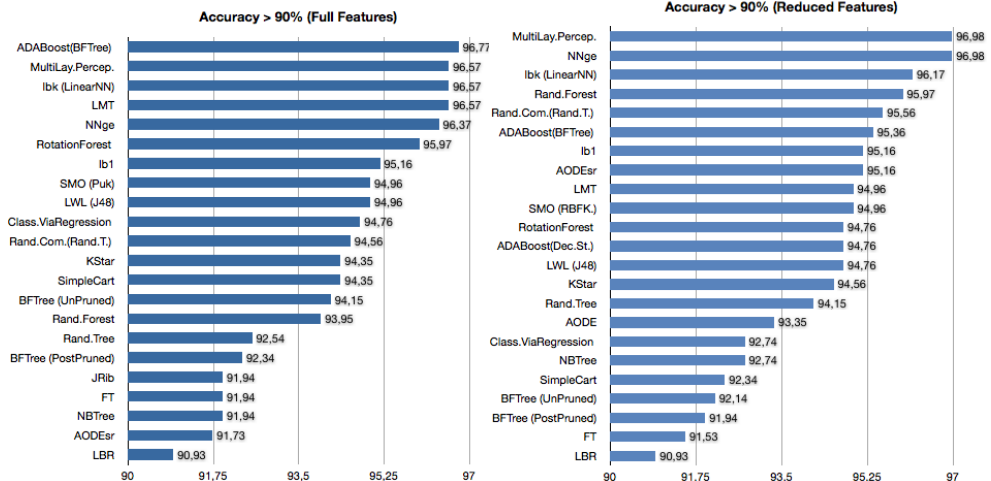
\includegraphics[width=\textwidth]{accuracy.png}
\caption{Preciznosti algoritama - sa svim atributima i bez}
\label{fig:acc}
\end{figure}

\begin{figure}[h!]
\centering
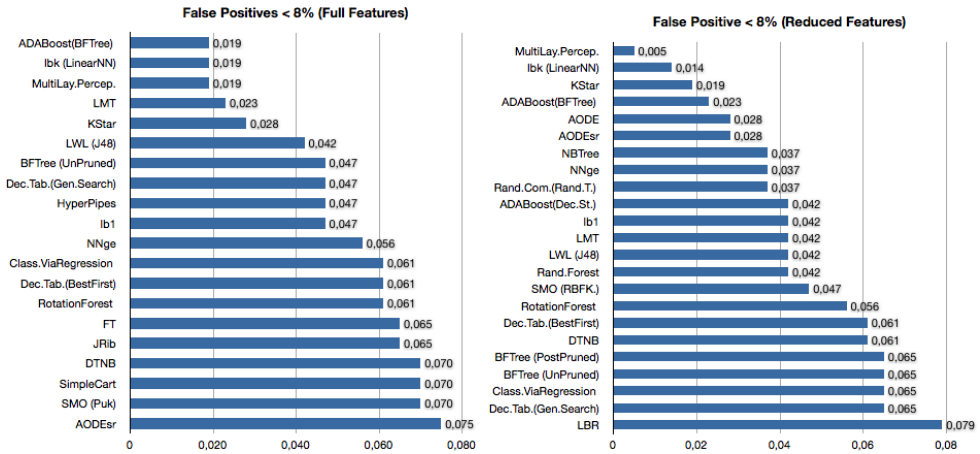
\includegraphics[width=\textwidth]{false_positive.png}
\caption{Lažno pozitivni - sa svim atributima i bez}
\label{fig:falsePos}
\end{figure}

Prema rezultatima dobijenim u  \cite{baca} vrlo je bitno da alat statičke analize ima malo lažno pozitivnih jer
u slučaju mnogo pogrešnih uzbuna programeri počinju da ignorišu te signale, ili još gore: kako bi izbegli upozorenja alata menjaju ispravan kod što dovodi do potencijalno
 novih greškaka. Na slici \ref{fig:falseNeg} se vidi da je ``NNge'' najbolji, što je i očekivano s obzirom na prilično
loše performanse što se tiče lažno pozitivnih.

\begin{figure}[h!]
\centering
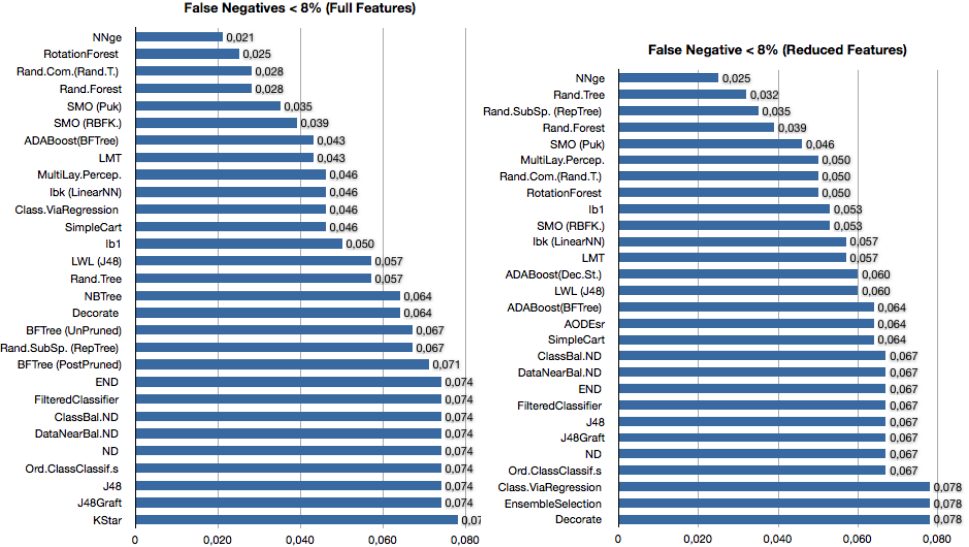
\includegraphics[width=\textwidth]{false_negative.png}
\caption{Lažno negativni - sa svim atributima i bez}
\label{fig:falseNeg}
\end{figure}

% ==============================================================================
\section{Primena mašinskog učenja u dinamičkoj verifikaciji}
\label{sec:dinamcikaPrimena}
% ==============================================================================

Priroda algoritama mašinskog učenja mnogo više odgovara problemima koji se sreću 
u dinamičkoj verifikaciji softvera. Stoga može se naći pregršt primena mašinskog 
učenja u ovoj oblasti. Radi potpunosti, u nastavku će biti opisana jedna od tih 
primena, koja se oslanja na učenje uslovljavanjem.


% ==============================================================================
\subsection{Onlajn testiranje korišćenjem učenja uslovljavanjem }
% ==============================================================================

Programi koji su reaktivni, naročito ako su distribuirani, mogu se ponašati nedeterministički. Neki faktori, poput redosleda završavanja niti nisu pod potpunom kontrolom testera, ali se njihovo ponašanje može modelovati stablom odlučivanja. Ipak, veličina tog stabla može da postane izuzetno velika za pretragu, pa se pribegava tehnikama onlajn testiranja.

Onlajn testiranje je tehnika u kojoj se kreiranje testa i njegovo izvršavanje rade u istom algoritmu. Može biti pogodnije od oflajn testiranja za reaktivne sisteme zato što se može dinamički prilagoditi za vreme izvršavanja tako da pokrije najrelevantnija ponašanja, umesto svih mogućih, što je obično nemoguće. Onlajn testiranje spada u skup testiranja baziranih na modelu (eng. model-based testing), gde tester koristi model da detektuje razlike između impelementacije pod testom (eng. implementation under test - IUT) i modela.

Razlikovaćemo poteze testera od IUTa. Akcije testera ćemo nazivati kontrolisane akcije, dok ćemo akcije IUTa nazivati posmatrane akcije. Greška usklađenosti nastaje kada IUT odbije kontrolisanu akciju modela ili kada model odbije posmatranu akciju IUTa.

Stanja modela su memorijske lokacije programa koje su preslikane u konačni skup vrednosti. 
Pravila ažuriranja su konačan skup funkcija koje preslikavaju vrednosti iz domena stanja u domen stanja. Pravilo ažuriranja $p$ može biti parametrizovano parametrima $\bar{x}$.
Instanciranje p[$\bar{x}$] ulaznim vrednostima $\bar{v}$ odgovarajućeg tipa, obeležava se p[$\bar{v}$].
Generalno, pravila ažuriranja mogu biti nedeterministička, tako da za isto ulazno stanje i vrednosti, može da ima različita izlazna stanja. Da bismo to modelovali, definišemo relaciju $[[p]] \subseteq Stanja \times Vrednost^n \times Stanja$.
Kada je p determinističko, [[p]] smatramo funkcijom [[p]]: $Stanja \times Vrednost^n  \rightarrow Stanja$

Čuvar $\varphi$ je formula koja zavisi od stanja. Može sadržati slobodne logičke promenljive $\bar{x} = x_1, x_2,..., x_n$ i takvo označavamo sa $\varphi(\bar{x})$. $\varphi$ je zatvoreno ako nema slobodnih varijabli. Zatvorena formula $\varphi$ ima istinitosnu interpretaciju u stanju $s \models \varphi$. Čuvano pravilo ažuriranja je par $(\varphi, p)$ i ono limitira primenu p na stanja i argumente koji zadovoljavaju $\varphi(\bar{v})$.

Model programa P sadrži sledeće komponente
\begin{itemize}
\item Prostor stanja $Stanja$
\item Prostor vrednosti $Vrednosti$
\item Inicijalno stanje $s_0 \in Stanja$
\item Konačni skup simbola akcija $\Sigma$ podeljen u dva disjunktna podskupa
	\item $\Sigma_c$ kontrolisanih akcija i
	\item $\Sigma_o$ posmatranih akcija
\item Familija $(\varphi_f, p_f) f \in \Sigma$ čuvanih pravila ažuriranja
	\item Arnost funkcije f je broj ulaznih parametara $p_f$
	\item Arnost reset pravila je 0 i $[[p_{Reset}]](s) = s_0$ za sve $s \models \varphi_{Reset}$
\end{itemize}
P je determinističko, ako za svako $f \in \sigma, p_f$ je determinističko. \\

Akcija $f$ ima oblik $f(v_1,...,v_n)$, gde je $f$ $n$-arni akcijski simbol a svako $v_i$ vrednost koja odgovara ulaznom parametru $p_f$. Kažemo da je akcija $f(\bar{v})$ dozvoljena u stanju $s$ ako $s \models \varphi(\bar{v})$. Primetimo dva specijanla slučaja: kada je reset uvek zabranjen $(\varphi_{Reset} = false)$, kada je definicija $p_{Reset}$ irelevantna, i slučaj kada je reset uvek dozvoljen $(\varphi_{Reset} = false)$, i tada $p_{Reset}$ mora da bude definisana tako da iz svakog stanja može da uspostavi početno stanje.

I IUT i model posmatramo kao interfejs automate (eng. interface automata) kako bismo formalno uspostavili vezu između njih \cite{interfaceAutomata}.
Interfejs automat M ima sledeće komponente:
\begin{itemize}
\item Skup stanja $S$
\item Neprazan podskup početnih stanja $S_init$ skupa $S$
\item Disjunktni skupovi kontrolisanih akcija $A_c$ i posmatranih akcija $A_o$
\item Dozvoljavajuće funkcije $\Gamma_c$ i $\Gamma_o$ podskupova $A_c$ i $A_o$, redom.
\item Prelazna funkcija $\sigma$ koja slika ulazno stanje i dozvoljavajuću akciju u izlazno stanje
\end{itemize}

Neka je P deterministčki model $(Stanja, Vrednosti, s_0, \Sigma, \Sigma_c, \Sigma_0, Reset, (\varphi_f, p_f)f \in \Sigma)$. Prema prethodnoj definiciji, intefejs automat P izgleda:

\begin{itemize}
\item $S_{[[P]]} = States$
\item $S^{init}_{[[P]]} = \{s_0\}$
\item $A^c_{[[P]]} = \{ f(\bar{v}) | f \in \Sigma^c, \bar{v} \subseteq Values \}$ 
\item $A^o_{[[P]]} = \{ f(\bar{v}) | f \in \Sigma^o, \bar{v} \subseteq Values \}$
\item $\Gamma^c_{[[P]]} = \{ f(\bar{v}) \in A^c_{[[P]]} | s \models \varphi_f(\bar{v}) \}$ 
\item $\Gamma^o_{[[P]]} = \{ f(\bar{v}) \in A^o_{[[P]]} | s \models \varphi_f(\bar{v}) \}$
\item $\sigma_{[[P]]}(s, f(\bar{v})) = [[P_f]](s, \bar{v}) (for f \in \Sigma, s \in States, s \models \varphi_f(\bar{v}))$
\end{itemize}

\noindent
Algoritam:

IUT I i model M, su oba predstavljeni kao interfejs automati.
Kako smo formalno definisali strukture modela, ostaje još da opišemo način izbora naredne akcije u algoritmu:
\begin{itemize}
\item Ukoliko nema mogućih akcija\\ prekini trenutni test. 
\item Ukoliko nema mogućeg izbora za kontrolisanu akciju\\ vrati posmatranu.
\item Ukoliko nema mogućeg izbora za posmatranu akciju\\ vrati kontrolisanu.
\item Inače\\ izaberi između kontrolisane i posmatrane akcije.
\end{itemize}

Algoritam prati težine transakcija u trenutnom testu. Sledeća kontrolisana akcija se bira iz nepraznog skupa dozvoljenih akcija koristeći datu strategiju:

Za ovaj problem koristićemo algoritam mašinskog učenja koji spada u učenje uslovljavanjem, o kome su osnove date ranije u radu. 
Cena testa se povećava srazmerno broju koraka kako bi se pokrio zadati procenat svih ponašanja. Iscrpno pokrivanje svih ponašanja je najčešće nemoguće. Umesto da posmatramo minimizaciju cene, možemo pretpostaviti da imamo fiksne resurse i da maksimizujemo procenat pokrivenih ponašanja. Bitno je da minimizujemo broj vraćanja u početno stanje (eng. backtracking), zato što to može biti skupa operacija. %ONLINE

Odabir sledeće akcije:
\begin{itemize}
\item Najjeftinija: \\
Biramo akciju koja najmanje košta, odnosno ima najveću nagradu.

\item Nasumična: \\
Biramo akciju na nasumičan način

\item Najmanje frekventna: \\
Klasičnu implementaciju familije algoritama učenja uslovljavanjem modifikujemo idejom anti-ant algoritma \cite{antiAnt} kako bi se izbeglo generisanje generacija redudantnih testova.
Akciju biramo nasumično, ali najveću verovatnoću ima stanje koje je inverzno proporcionalno njegovoj ceni. To znači da su manje frekventne akcije favorizovane.
Drugim rečima, ako potencijalne sledeće akcije obeležimo sa $(a_i)_{i < k}$ za neko k, i cene $(c_i)_{i < k}$, onda će verovatnoća za izbor akcije $a_i$ biti $c_i^{-1} / \sum_{j!=i}^{} c_j^{-1}$.
\end{itemize}

U radu \cite{online-testing-with-reinforcement-learning} se mogu videti primeri eksperimenta sa sva tri pristupa.


% ==============================================================================
\section{Zaključak}
\label{sec:zakljucak}
% ==============================================================================

\par Verifikacija softvera je veoma važna jer su moguće posledice neispravnog softvera ogromnih razmera. Tehnike mašinskog učenja se brzo u\-sa\-vr\-ša\-va\-ju i pokazuju izuzetno dobre rezultate, pa je prirodno razmišljati o njihovim mogućim primenama na verifikaciju softvera.

\par Od primena mašinskog učenja na statičku verifikaciju softvera prikazane su tehnike formalne verifikacije, učenje statičkog analizatora i kako od izvornog koda doći do istreniranih modela, a od primena na dinamičku verifikaciju prikazana je tehnika učenja uslovljavanjem na onlajn testiranjima. U formalnoj verifikaciji se na osnovu skupa testova indukuju teorije koje bi trebalo da se poklapaju sa specifikacijom programa. Proces korišćenja generisanja kontraprimera, koji je obrađen u \ref{subsec:staticki-analizator} је inovativan pristup regularizaciji modela mašinskog učenja, koji se do sada nije javljao u naučnim radovima. U \ref{subsec:pregled} dat je primer prikupljanja podataka za trening i upoređivanje rezultata različitih algoritama koji imaju za cilj statičku detekciju grešaka. Kod onlajn testiranja se u isto vreme kreira i izvršava test i treba pokriti što više ponašanja sa fiksnim resursima. Učenje uslovljavanjem navodi da se ide na nefrekventne testove, a uz to postoje dodatni parametri, kao što je kazna ako se vrati u početno stanje.


\addcontentsline{toc}{section}{Literatura}
\appendix
\bibliography{seminarski}
\bibliographystyle{plain}

\end{document}